\documentclass[11pt]{beamer}
\usetheme{Copenhagen}
\usepackage[utf8]{inputenc}
\usepackage{amsmath}
\usepackage{amsfonts}
\usepackage{amssymb}
\usepackage{graphicx}
\usepackage{subcaption}
\usepackage[backend=bibtex,style=ieee]{biblatex}
\addbibresource{abe-blockchain.bib}
\author{Andrei Cristian}
\title{Using ABE to Secure Blockchain Transaction Data}
\setbeamercovered{transparent} 
\setbeamertemplate{navigation symbols}{} 
%\logo{} 
%\institute{} 
%\date{} 
%\subject{} 
\begin{document}

\begin{frame}
\titlepage
\end{frame}

\begin{frame}{Table of Contents}
\tableofcontents
\end{frame}

\section{Introduction}
\begin{frame}{Introduction}
\begin{itemize}
	\item Blockchain technology is increasingly being adopted as a trusted platform to support business functions including trusted and verifiable transactions, tracking, and validation.
	\item Most business use-cases require privacy and confidentiality for data and transactions $\Rightarrow$ \textbf{Private blockchain solutions} $\Rightarrow$ Unable to take full advantage of the capabilities, benefits and infrastructure of public blockchain systems.
	\item \textbf{Attribute-Based Encryption} security solution built on private-over-public (PoP) blockchain $\Rightarrow$ Businesses will be able to \textbf{restrict access}, \textbf{maintain privacy}, \textbf{improve performance}, while still being able to benefit from the distributed trust of public blockchains.
\end{itemize}
\end{frame}

\begin{frame}[allowframebreaks]{Public and Private Blockchains}
\begin{itemize}
	\item Similarities\cite{jayachandran}:
	\begin{enumerate}
		\item both are decentralized peer-to-peer networks, where each participant maintains a replica of a shared append-only ledger of digitally signed transactions;
		\item both maintain the replicas in sync through a protocol referred to as consesnsus;
		\item both provide certain guarantees on the immutability of the ledger, even when some participants are faulty or malicious.	
	\end{enumerate}
	\item The main distinction between public and private blockchain is related to who is allowed to participate in the network.
	\item One of the drawbacks of the public blockchain is the substantial amount of computational power to maintain a distributed ledger at a large scale to achieve consensus, in which each node in a network must solve a complex, resource-intensive cryptographic problem - called Proof of Work (PoW)\cite{nakamoto2008} to ensure all are in sync.
	\item Another disadvantage is the openness of public blockchain, which implies little to no privacy protection for transactions and only supports a weak notion of security.
	\item Many people believe private blockchains could provide solutions to many financial enterprise problems, that public blockchains do not, such as abiding by regulations such as Health Insurance Portability and Accountability Act (HIPPA), anti-money laundering (AML) and know-your-customer (KYC) laws, etc.
	\item Private blockchain is usually much faster, cheaper and respects the company's privacy.
	\item  Private blockchains also provide more control power over the participants in the blockchain.
	\item \textbf{Cross-chain} functionality aims to combine the best features of different blockchain systems\cite{liebkind2018}, both private and public, for the purposes of exchanging value across disconnected ecosystems.
	\item None of existing solutions clearly addressed the problem of applying access control policies to enforce data privacy protection on transaction secrets.
	\item For example, when using smart contract solutions, e.g. Ethereum\cite{ethereumweb}, for procurement in supply-chain, transaction parameters such as product name, quantity, price, purchasing terms, shipping options, address, etc. could all be \textbf{sensitive business secrets}. They should be only viewable for relevant stakeholders. 				\item Hyperledger\cite{cachin2016} addresses this problem by relying on a TA approach to build permission groups for data access control. However, data access must be \textbf{predefined} which is not suitable for complex and dynamic businesses logic that require dynamic access control.
	\item \textbf{RBAC} is \textbf{incompatbile} with the distributed nature of blockchain operations where transaction data are mobile and shared by multiple blockchain participants.
\end{itemize}

\end{frame}

\begin{frame}{POP architecture}

\begin{figure}[!ht]
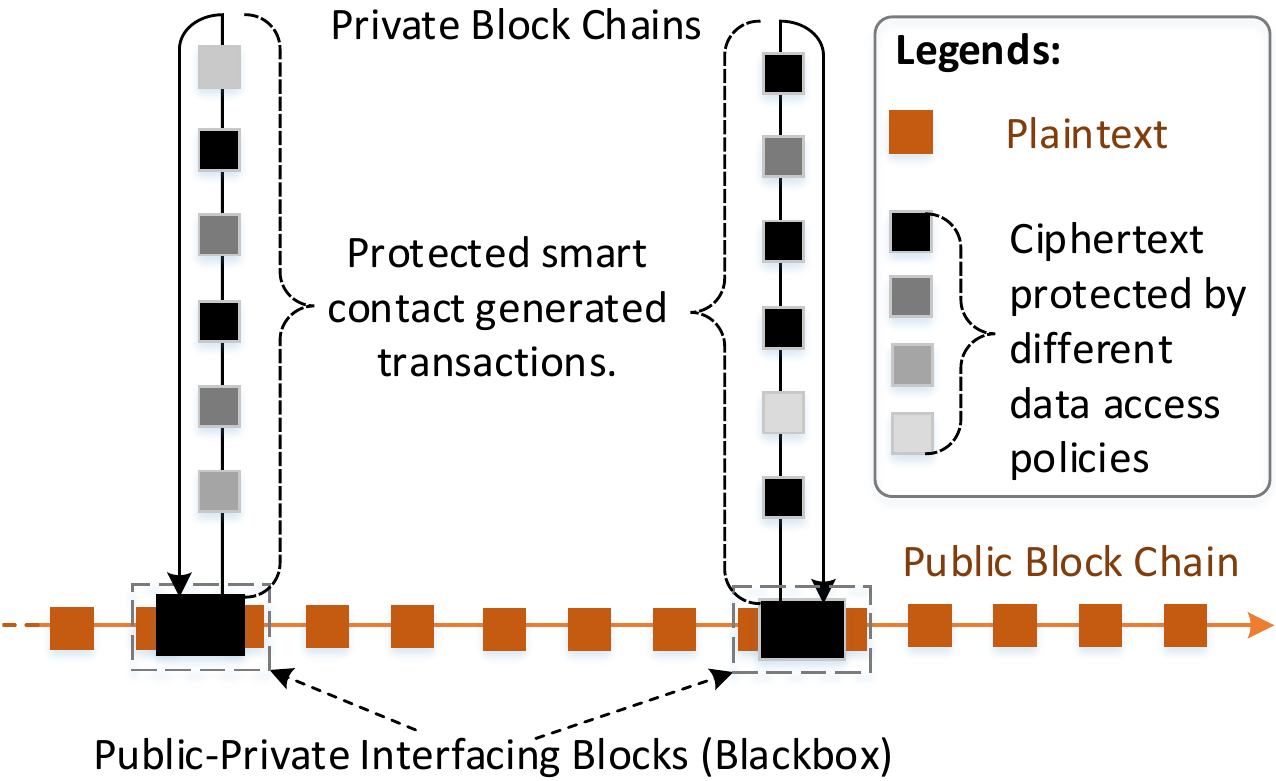
\includegraphics[scale=0.25]{pop.png}
\caption{Illustration of PoP blockchain architecture.}
\label{fig:poparchitecture}
\end{figure}

\end{frame}

\begin{frame}[allowframebreaks]{ABE over PoP Blockchain}
\begin{itemize}
	\item PoP architecture is presented in Figure \ref{fig:poparchitecture}.
	\item Applying ABE on an off-chain basis means it can inter-operate with the public blockchain without interference.
	\item  Private blockchains transactions can be much
\textbf{less computationally intensive} and provide \textbf{superior performance} since they do not have to be verified by all participants.
	\item Businesses are able to choose the private blockchain solution that \textbf{best suits their needs} independently from the public blockchain.
	\item Each private blockchain can be viewed as a \textbf{protected state channel}.
	\item The integrity of a private blockchain can be validated and checked in ciphertext and in aggregate by all public blockchain participants.
	\item The public blockchain infrastructure is leveraged to provide \textbf{validation} and \textbf{immutability} for the entirety of the private blockchain state channel.
	\item This can take
the form of the final private blockchain transaction result, or a hash of the entire private blockchain $\Rightarrow$ distributed trust on the public chain is \textbf{not necessary} for the private blockchain.
	\item \textbf{ABE} provides \textbf{data privacy} for the private blockchain state channel.
	\item Only participants with the appropriate permissions and corresponding ABE attribute private keys can view and validate their relevant blocks in the private block chain.
	\item It provides the benefits of private blockchains in terms of privacy without requiring the deployment of trusted nodes or multiple verification nodes.
	\item It essentially minimizes the entry cost businesses in adopting blockchain solutions.
\end{itemize}
\end{frame}

\begin{frame}[allowframebreaks]{The PoP Solution}
In summary, the presented PoP solution has the following main features:
\begin{itemize}
	\item It is a decentralized trust model for key management of ABE-based data access control. Using this approach, it can incorporate access control policies into ciphertext to protect content of smart contracts.
	\item It is a privacy-preserving messaging protocol to allow private blockchain participants to interact with the smart contract that can generate a private blockchain. This chapter illustrates how to use this protocol based on a supply-chain procurement application.
	\item The solution provides two smart contracts: \textbf{PPP} (Public Parameters and Policies) to establish attribute based security trust model and \textbf{ppSCM} to provide secure data access control based on ABE scheme.
	\item A comprehensive security and performance analysis is presented based on the presented PPP scheme. The presented solution is practical that can significantly reduce the effort and cost to establish dedicated and isolated private blockchains.


\end{itemize}

\end{frame}

\section{System and Models}
\begin{frame}{System and Models}
\begin{itemize}
	\item To illustrate the presented solution, in Figure \ref{fig:supplychain} it is used a supply chain example based on \textbf{Block-Chain Technology}(BCT), which involves multiple parties.
	\item The potential of having all the information written in a blockchain allows the creation of an \textbf{authoritative record} that can be used to \textbf{automatically} establish smart contracts.
	\item Because the information is registered on a distributed database, it makes it \textbf{tamper-resistant} and \textbf{fosters greater trust} in the trade network.
\end{itemize}
\end{frame}

\begin{frame}{Supply chain example}
\begin{figure}[!ht]
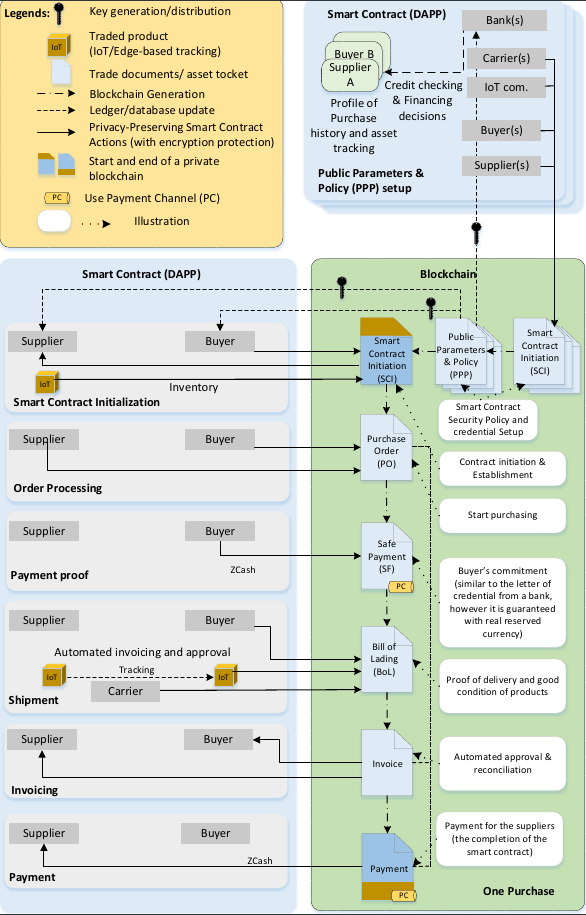
\includegraphics[scale=0.21]{supplychainexample.png}
\caption{A supply chain scenario using IoT devices, blockchain, and data encryption protections.}
\label{fig:supplychain}
\end{figure}
\end{frame}

\begin{frame}{Legends and Smart Contract interaction with Blockchain}
\begin{figure}[!ht]
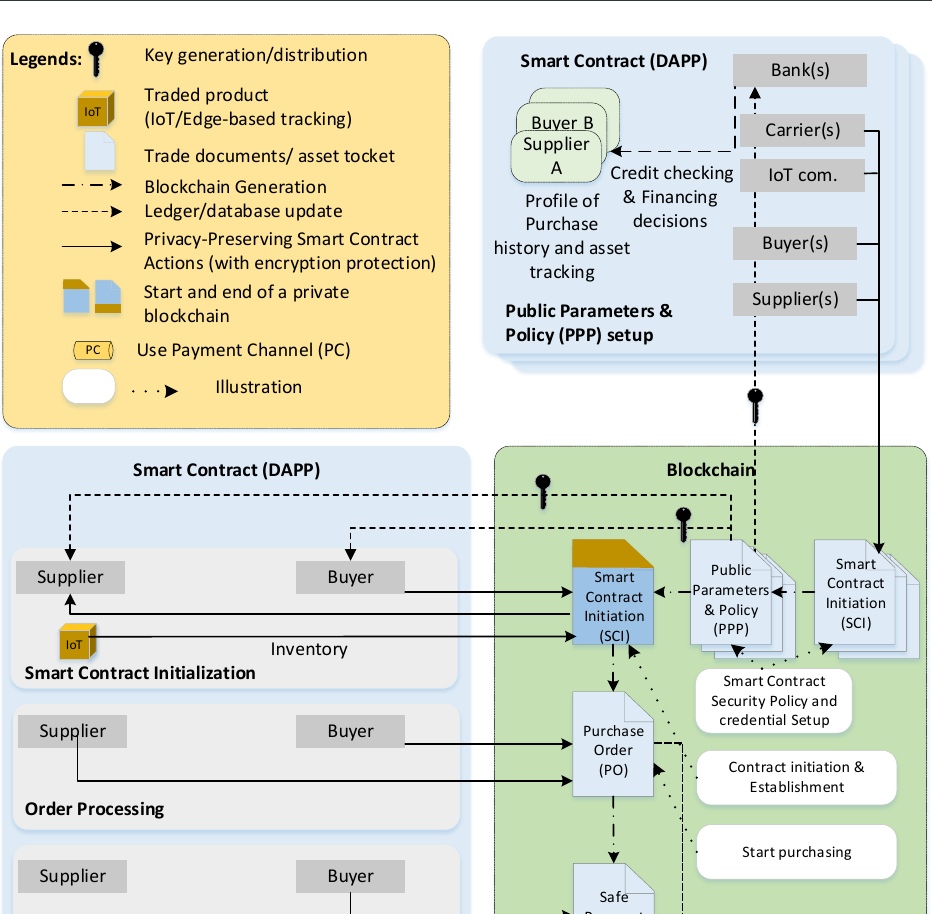
\includegraphics[scale=0.20]{supplychainlegendsscb.png}
\caption{Zoom-in on Legends and interaction of the first smart contract with the blockchain}
\label{fig:supplychainlegendsscb}
\end{figure}
\end{frame}

\begin{frame}{Smart Contract interaction with Blockchain}
\begin{figure}[!ht]
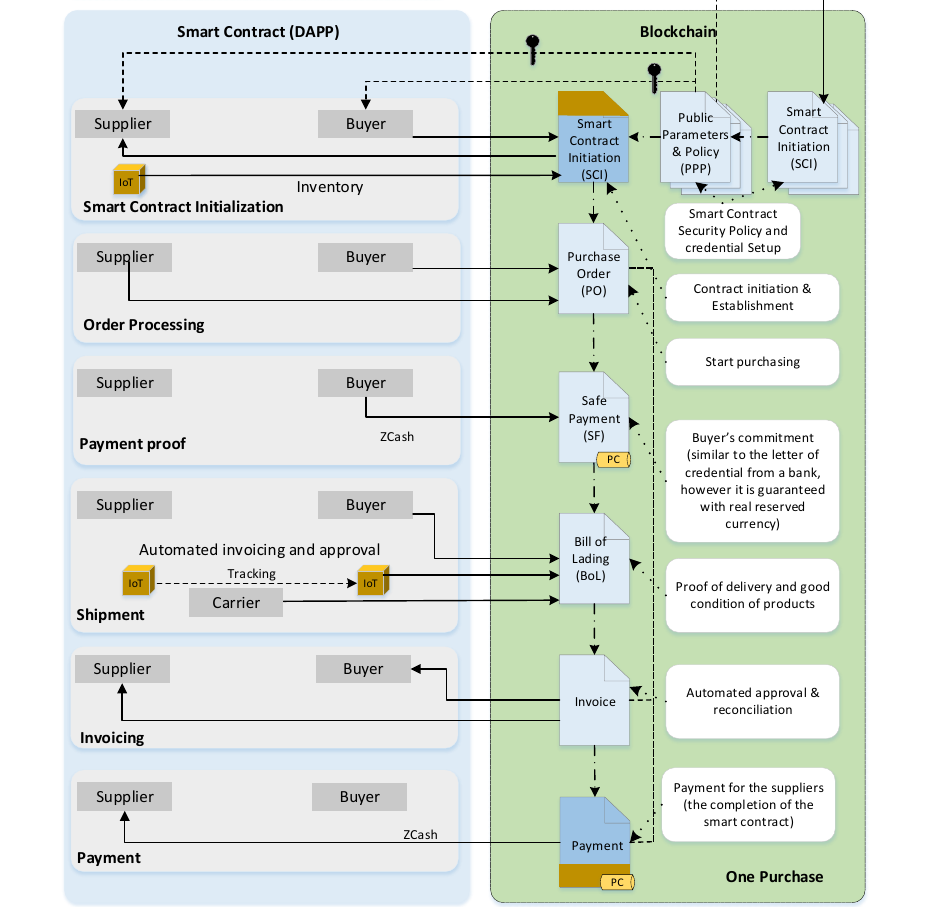
\includegraphics[scale=0.20]{supplychainscb.png}
\caption{Zoom-in on the interaction of the second smart contract with the blockchain}
\label{fig:supplychainscb}
\end{figure}
\end{frame}

\begin{frame}[allowframebreaks]{BCT-supported purchase related transaction using DApp}
The left side of the figure present a BCT-supported purchase related transaction by using Ethereum’s Decentralized App (DApp) solution involves 4 main procedures based on supply-chain operation procedures:
\begin{itemize}
\item \textbf{Order Processing}:
\begin{itemize}
	\item The order-processing workflow starts with a PO from the buyer. Within the blockchain, once created, the PO is time-stamped and can become a valid document whose clauses can be executed \textbf{only if valid}, due to the programming features of smart contracts.
	\item Assuming delivery documents can also be registered on it, the metadata of the invoice, PO and bill of lading could be matched automatically due to the smart contracts feature, which \textbf{ensures consistency between price and quantity} in all three documents (i.e. three-way-match), permitting an \textbf{automated} and \textbf{fast invoice approval}.
	\item The entire history of the transactions offers \textbf{perfect audibility}, and \textbf{trust between parties} is provided by the \textbf{immutability of the data} entered in a blockchain.
\end{itemize}	  

\item \textbf{Shipment}:
\begin{itemize}
	\item \textbf{IoT-based tracking capability} is a critical component for this procedure.
	\item Keeping track of the \textbf{material flow} at each step, along with the corresponding \textbf{paper flow}, is a major undertaking that \textbf{requires manual processes} that are subject to \textbf{human error}, \textbf{loss}, \textbf{damage} or even \textbf{theft} and \textbf{fraud}.
	\item Another potential application is provided by smart contracts and cryptographic multi-signatures and product content protection for all the various documentation and processing stages involved in a trade transaction.
	\item In such a blockchain-based IoT, there is the possibility of maintaining \textbf{product information}, its \textbf{history}, \textbf{product revisions}, \textbf{warranty details} and \textbf{end of life}, transforming the blockchain into a distributed and trusted blockchain.
\end{itemize}


\item \textbf{Invoicing}:
\begin{itemize}
	\item Blockchain-based services can register the invoice-related information on a blockchain in order to \textbf{avoid} \textbf{duplicates} and \textbf{fraud} across the network.
	\item As explained by \cite{hofmannstrewebosia}, each invoice would be distributed across the network, hashed and time-stamped in order to create a \textbf{unique identifier}.
	\item If a supplier tried to sell same invoice again through the network, that invoice would indicate a previous instance of financing to all parties, and the \textbf{double financing would be avoided}.
	\item The \textbf{integration with the payment system} is given by the ability of smart contracts to \textbf{take control over an asset} registered on a blockchain (e.g. crypto-cash) and \textbf{automatically trigger the payment}.
\end{itemize}

\item \textbf{Payment}: 
\begin{itemize}
	\item Developed to create a purely peer-to-peer version of electronic
cash to allow online payments, \textbf{payments are the first application of BCT}.
	\item With the use of Bitcoin or similar cryptocurrencies in a B2B scenario, buyer and supplier could \textbf{transact without any intermediaries} (e.g. banks) and with \textbf{very small transaction fees}.
	\item Blockchain solutions could create \textbf{more efficient payment processes} between banks, eliminating the need for each institution to \textbf{maintain} and \textbf{reconcile their own ledger}.
\end{itemize}

\end{itemize}

\end{frame}

\begin{frame}[allowframebreaks]{Privacy problem}
\begin{itemize}
\item The described smart contract \textbf{does not provide privacy protection} for transaction contents processed by smart contracts.
\item Two additional modules (incorporated into original supply-chain procedures):
\begin{enumerate}
	\item \textbf{Smart contract initialization}: 
	\begin{itemize}
		\item sets up the initial smart contract credentials such as agreed data access control policies for each step of smart contract;
		\item initiates the off-chain operation, in which we start a private blockchain at this point.
	\end{itemize}
	\item \textbf{Payment proof}:
	\begin{itemize}
		\item the private chain can also incorporate public blockchain evidence into the private blockchain;
		\item the addition of the payment proof procedure is to utilize the payment channel feature of public blockchains to \textbf{prove the buyer has sufficient money} to pay for the purchased product;
		\item  the buyer first pays for the product to a Escrow account, and once the product is landed, the cashed money will be delivered to the supplier to close the blockchain based purchase.
	\end{itemize}
\end{enumerate}
\end{itemize}
\end{frame}

\begin{frame}[allowframebreaks]{Smart Contracts}
\begin{itemize}
\item In Bitcoin, the concept of \textit{“scripting”} has already existed, which is actually \textbf{a weak version} of smart contract.
\begin{itemize}
	\item it lacks Turing-completeness, thus does not nearly support everything;
	\item it is value-blinded;
	\item it lacks state, UTXO can either be spent or not, there is no way to keep other states except for these two;
	\item it is blockchain blinded.
\end{itemize}
\item Ethereum smart contract is to build a decentralized application to create a blockchain with a build-in Turing complete programming language.
\item Smart contract means is defined to be a cryptographic “boxes” that contain value and only unlock it if certain conditions are met.
\item A smart contract will also be stored in the blockchain and can be retrieved by its address and integrity can be guaranteed as well.
\item With smart contract, one can express logics such as “only after April 17th, 2018, can the document be sent to A”.
\item In the presented supply-chain example in Figure \ref{fig:supplychain}, two smart contracts are involved:
	\begin{enumerate}
	\item \textbf{public blockchain smart contract}: the smart contract on the right side box includes multiple stake holders providing supply-chain services to settle down a \textbf{PPP} (Public Parameters and Policies).\\A PPP describes what encryption \textbf{public parameters} will be used for \textbf{data privacy protection}, who may serve as a \textbf{trusted party} for \textbf{data access control management} for running private blockchains, and what \textbf{security policies to be enforced} in the private blockchain. \textbf{We can treat PPP as a template};
	\item \textbf{private blockchain smart contract}: the smart contract on the left side of Figure \ref{fig:supplychain} represents a one purchase between a supplier and a buyer. In addition, an \textbf{IoT company} can be involved to provide \textbf{product tracking and inventory}.
	\end{enumerate}
\end{itemize}
\end{frame}

\begin{frame}{ABE-Enabled ABAC}
\begin{itemize}
\item ABE is a way to implement attribute-based access control, in which,
data will be encrypted and a data owner could define an access policy describing what attributes the data users need to own in order to get access of the data.
\item Presentation of an extended Lewko's scheme \cite{lewkowaters} by adding \textbf{distributed trust management} to allow multiple parties to \textbf{collaboratively establish the trust} and \textbf{distribute secret keys}.
\item The following described Federated Authority Setup and Federated KeyGen protocols are \textbf{newly proposed}.
\end{itemize}

\end{frame}

\begin{frame}[allowframebreaks]{Comparing existing blockchain data privacy protection solutions}

The presented approach has the following important features compared to existing blockchain data privacy protection solutions:

\begin{itemize}

\item \textbf{Distributed and mobile}: every participant in the system can serve as a trust authority to issue attributes and corresponding private keys for private blockchain participants; the access control policy is associated with ciphertext, which can be freely shared among blockchain stakeholders without needing an access control infrastructure for data management.
\item \textbf{Federated}: attributes can be shared among private blockchain participants. This also means that the scheme allows a coalition to be established for a private blockchain for attributes and corresponding private keys generation. The coalition can prevent single point failure issue as well resisting to $n - 1$ collusion problem, where n is the size of the coalition.
\item \textbf{Provides interoperability feature}: attributes and corresponding private keys generated from different trust authorities can be used together to form a data access control policy.\\For example, Alice can use her own generate private key for attribute $A_1$ and another attribute $A_2$, which is generated by Bob to decrypt a data protected by data access policy enforced by the policy \{$A_1$ AND $A_2$\}.
\end{itemize}

\end{frame}

\begin{frame}[allowframebreaks]{Security Policy}

A typical security policy should include multiple descriptive terms(i.e., attributes) such as:
\begin{center}
$\mathcal{P}1=$The \textbf{pricing} and \textbf{quantity} can be accessed by\\the \textbf{supplier} and the \textbf{buyer}.
\end{center}
In this policy, 'pricing' and 'quantity' are accessing objects, and 'supplier' and 'buyer' are attributes describing accessing subjects. These attributes can be used as public encryption keys. In each block created by the private blockchain, data are encrypted using one or multiple data access policies.

\begin{figure}
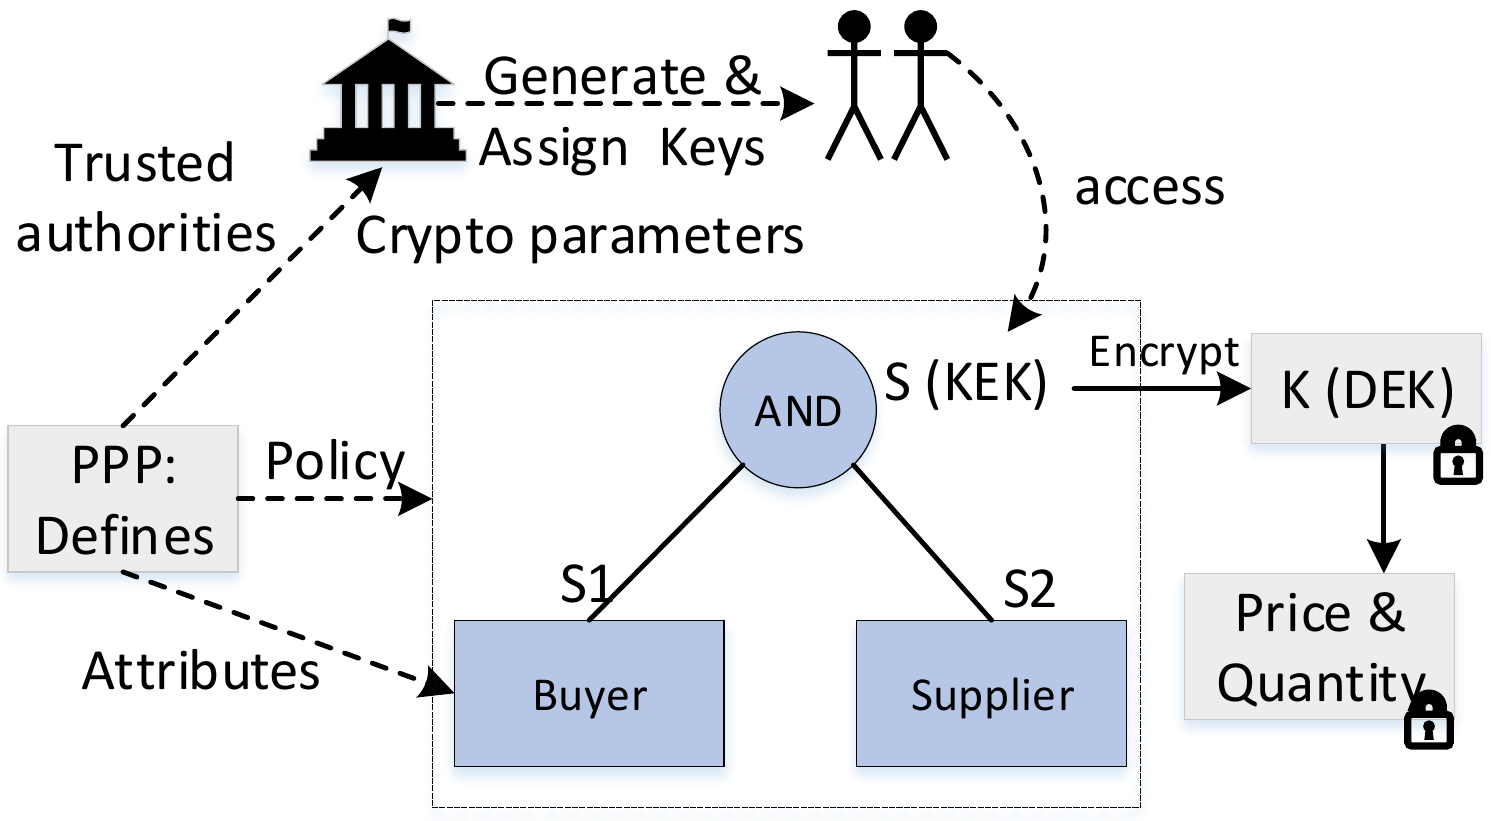
\includegraphics[scale=0.2]{abacsetup.png}
\caption{Attribute(or policy)-based access control setup.}
\label{fig:abacsetup}
\end{figure}

\begin{enumerate}
\item The policy $\mathcal{P}1$ is presented in Figure \ref{fig:abacsetup}, which is called Policy Tree (PT).
\item A PT is constructed by attributes at the leaves and intermediate nodes are logical gates.
\item Using secret sharing scheme, a tree-root level secret \textit{s} can be used as a Key-Encrypting Key (KEK) to protect at symmetric key \textit{K} as the Data Encrypting-Key (DEK) to protect data such as the values of price and quantity.
\item The smart contract generated PPP defines attributes and policies for a particular application, and trusted parties, and crypto parameters used for key generation and encryption in the private blockchain.
\end{enumerate}

\end{frame}

\begin{frame}[allowframebreaks]{Scheme Construction}
\begin{itemize}
\item Lewko's scheme requires users to derive their private key from one trusted authority to allow them to use the same attribute and corresponding private key to decrypt a ciphertext.
\item Extension of Lewko's solution by adding multi-authority key generation scheme - \textit{federated authority setup} and \textit{federated key generation}, for an attribute and corresponding private key is generated by multiple authorities.
\item Only if \textbf{all} involved trusted authorities got compromised, e.g., using collusion attack, can they derive the private key for a user.
\item Considering the heavy computation overhead, part of the encryption and decryption computation is outsourced to the edge nodes. The following is the outsourced version of the scheme.
\item \textbf{Global Parameters Setup$(\lambda)\rightarrow GP$:}
	\begin{itemize}
	\item The Global Parameter (GP) can be established in advance by a well-known organization,e.g., in the supply-chain industry.
	\item Since the GP is publicly known, it is not critical for which party to generate the GP.
	\item The organization selectes a composite \textit{Bilinear} group G or order $N=p_1p_2p_3$.
	\item $GP=\{N,g_1,H:\{0,1\}* \rightarrow G\}$, where $g_1$ is a generator of group $G_{p_1}$ and the hash function $H$ is mapping function that maps a global identifier to an element of group $G$.
	\item This algorithm might be run multiple times by different entities so as to generate multiple candidate global parameters in the candidate public parameters and policies (PPP).
	\end{itemize}
\item \textbf{Authority Setup$(GP)\rightarrow MPK,MSK$:}
	\begin{itemize}
	\item Each blockchain participant can serve as a trusted authority for key generation.
	\item Based on the GP, they need to choose and publish a set of public parameters, i.e., a master public key $MPK$, which can be later used for private key generation.
	\item For each attribute $A_i$ that is managed by the authority, the authority $j$ chooses randomly $\alpha_i,y_i \in \mathcal{Z}_N$ and publishes $MPK_j=\{e(g_1,g_2)^{\alpha_i}, g_1^{y_i},\forall i\}$ as the public key.
	\item The corresponding master private key is $MSK_j=\{\alpha_i,y_i,\forall i\}$.
	\end{itemize}
	
\item \textbf{Federated Authority Setup$(GP,AAS)\rightarrow\hat{MPK},\hat{MSK}$:}
	\begin{itemize}
	\item Using Lewko's scheme, each authority can generate a private key for a given attribute.
	\item To relax the requirement that states that the same authority must be used for the private keys to be derived, multiple authorities must be involved for private key generation to prevent single point failure issue.
	\item If there are $n$ federated authorities, then this scheme is resistant to $n - 1$ authority collusion problem.
	\item The federated authority setup algorithm is run when multiple attribute authorities need to generate the public key and private key for their shared attribute(s).
	\item For simplicity, we assume there are $n$ attribute authorities in the set $AAS$.
	\item $AAS = \{AA_1,AA_2,\cdots,AA_n\}$.
	\item $AA_i$ will generate $\alpha_i,y_i \in \mathcal{Z}_N$.
	\item Each $AA_i$ will generate an individual master private key $MSK_i = \{\alpha_i,y_i,\forall i\}$.
	\item $AA_{i-1}$ will send the individual master public key to $AA_i$ as:
	\[MPK_{i - 1\rightarrow i} = \{e(g_1,g_1)^{\Sigma_{j = 2}^i y_{j - 1}}\}\]
	\item $AA_i$ will calculate:
	\[MPK_{i\rightarrow i+1} = (e(g_1,g_1)^{\Sigma_{j = 2} ^ i \alpha_{j - 1 }})^\alpha_i, (g_1^{\Sigma_{j = 2}^i y_{j - 1}})^y_i.\]
	\item The final federated master public key and private key for an attribute is defined as follows:
	\[\hat{MPK} = \{e(g_1,g_1)^{\Sigma_{j = 1}^n \alpha_j}, g_1^{\Sigma_{j = 1}^n y_j}\},\]
	\[\hat{MSK} = \{\sum_{j=1}^n \alpha_j, \sum_{j = 1}^n y_j\}.\]
	\end{itemize}

\item \textbf{Encrypt$(M, (A, \rho), GP, \{MPK\},\hat{MPK} \rightarrow CT$:}
	\begin{itemize}
	\item \textit{M} is a message.
	\item \textit{A} is an $n \times \ell$ access matrix.
	\item $\rho$ maps its rows to attributes.
	\item For each row in \textit{A}, the algorithm chooses a random number $r_x \in \mathcal{Z}_N$.
	\item A random vector $w \in \mathcal{Z}_n^\ell$ with 0 being the first entry is chosen randomly.
	\item $\omega$ denotes $A_x \cdot \omega$.
	\item The data owner chooses $s \in \mathcal{Z}_N$ and a vector $v \in \mathcal{Z}_N^\ell$ randomly, where $s$ is its first entry.
	\item $\lambda_x = A_x \cdot v$ with $A_x$ being the $x$\textsuperscript{th} row of the matrix $A$.
	\item The ciphertext is as follows:
	\[CT=<C_0, C_{1,x}, C_{2,x}, C_{3,x}>, \quad \textit{where} \]
	\[C_0 = Me(g_1,g_1)^s, \quad C_{1,x} = e(g_1,g_1)^{\lambda_x} e(g_1,g_1)^{\alpha_{\rho(x)} r_x},\]
	\[C_{2,x} = g_1^{r_x}, \quad C_{3,x} = g_1^{y_{\rho(x)} r_x} g_1 ^{\omega_x}, \forall x.\]
	\item CT is the ciphertext of DEK, which is used to encrypt data object \textit{o} in the blockchain protocol.
	\item In this encryption protocol, the encryptor needs to identify which master public key parameters are used for each involved attribute.
	\item Later, a decryptor can use private keys generated from corresponding public keys.
	\end{itemize}

\item \textbf{KeyGen$(GID, i, \{MSK\}, GP) \rightarrow SK_{i, GID}$:}
	\begin{itemize}
	\item In PoP, the \textit{GID} can be an address that is used to identify the blockchain participant.
	\item For a global identifier \textit{GID} with attribute \textit{i} belonging to an authority, the authority generates the following private key
	\[SK_{i, GID} = g_1^{\alpha_	i} H(GID)^{y_i}.\]
	\item Using the \textit{KeyGen} scheme, an authority can generate private keys for other blockchain participants.
	\end{itemize}

\item \textbf{Federated KeyGen$(GID, i, \{MSK\}, \hat{MSK}, GP) \rightarrow SK_{i, GID}$:}
	\begin{itemize}
	\item The federated key generation algorithm is run when multiple attribute authorities need to generate the private key for an attribute shared among multiple users.
	\item Assume that $AAS = \{AA_1, AA_2, \cdots, AA_n\}$.
	\item $AA_i$ will generate $g_1^{\alpha_i} H(GID)^{y_i}$.
	\item $AA_{i - 1}$ will send $AA_i$ the private key component:
	\[ SK_{i - 1 \rightarrow i} = g_1^{\Sigma_{j = 1}^i \alpha_{j - 1}} H(GID)^{\Sigma_{j = 2} ^ i y_{j - 1}}.\]
	\item Then, $AA_i$ will calculate
	\[ SK_i = (g_1^{\Sigma_{j = 2}^i \alpha_{j - 1}})^{alpha_i} (H(GID)^{\Sigma_{j = 2}^i y_{j - 1}})^{y_i}\].
	\item The final secret key of the shared attribute for the user GID is as follows:
	\[ SK_{i,GID} = g_1^{\Sigma_{j = 1} ^ n \alpha_j}H(GID)^{\Sigma_{j = 1} ^ n y_j}.\]
	\end{itemize}
	
\item \textbf{Decrypt$(CT, \{SK_{i,GID}\}, GP) \rightarrow M$:}
	\begin{itemize}
	\item Assume that the ciphertext is encrypted under an access matrix $(A, \rho)$.
	\item If the decrypt holds the private key $\{SK_{\rho(x), GID}$ for a subset of rows $A_x$ of $A$ satisfying that $(1, 0, \cdots, 0)$ is in the span of these rows, then the plaintext message $M$ can be obtained in the following way:
	\[C_{1,x} \cdot e(H(GID), C_{3,x})/e(SK_{\rho(x),GID}, C_{2,x}) = \]
	\[=e(g_1,g_1)^{\alpha_x}e(H(GID), g_1)^{\omega_x}.\]
	\item The decryptor chooses constants $c_x \in \mathcal{Z}_N$ so that $\Sigma_x c_x A_x = (1, 0, \cdots, 0)$ and computes
	\[\prod_x (e(g_1, g_1)^{\lambda_x} e(H(GID), g_1)^{\omega_x})^{c_x} = e(g_1, g_1)^S.\]
	\item To verify the transaction including encrypted data, the decryption algorithm will be called.
	\end{itemize}

\end{itemize}

\end{frame}

\begin{frame}[allowframebreaks]{Offloaded Encryption and Decryption}

\begin{itemize}
\item Considering participant running DApp on mobile devices, ABE based computation can be potentially intensive for mobiles.
\item $\Rightarrow$An ABE offloading model that can significantly reduce the computation overhead on mobiles.
\item Assumption that an edge cloud node can assist mobiles to perform offloading functions.
\item \textbf{Encrypt}: similar to the encryption presented in \textit{Scheme Construction}, but only $C_0, C_1$ are calculated by the data owner (mobile device), and $C_2,C_3$ are calculated by the edge node.
\item \textbf{Decrypt}: similar to the decryption presented in \textit{Scheme Construction}, but the private key holder only needs to calculate $e(SK_{\rho(x), GID}, C_{2,x})$. The edge node will calculate $C_{1,x}\cdot e(H(GID),C_{3,x})$.
\end{itemize}

\end{frame}

\begin{frame}{Security Model}
\begin{itemize}
\item PoP assumes that blockchain participants are curious, selfish, and greedy, and they want to learn business secrets incorporated into blockchains.
\item They may collude to share their secrets to gain additional data access capabilities that should not assigned to them.
\item Moreover, they may drop off from blockchain creating procedure to take the goods without paying for it.
\end{itemize}
\end{frame}

\section{PoP System Models}
\begin{frame}[allowframebreaks]{Access System Construction}
\begin{itemize}
\item \textbf{Definition 1}(Contract)
	\begin{itemize}
	\item A smart contract \textit{C} is defined by a procedure $C = \{T\}$.
	\item The procedure specifies a set of interdependent transactions among contract subjects (or participants) in group \textit{G}.
	\end{itemize}
\item \textbf{Definition 2}(Transaction)
	\begin{itemize}
	\item A transaction defines a sequential atomic data actions $\{a\} \in A = \{\mathit{read,write,change}\}$.
	\item Each action \textit{a} is restricted by a privilege $\alpha(a,T): \mathcal{P}(a,T) \longmapsto S_{a,T}$.
	\item The privilege $\alpha(a, T)$ are defined by capabilities such as $\{$\textit{can, cannot, restricted by/to}$\}$.
	\end{itemize}
\break
\item \textbf{Definition 3}(Subject)
	\begin{itemize}
	\item A subject $s \in S$ or \textit{G} ( here \textbf{S} is a subset of subjects and \textbf{G} is the overall group and includes all the subjects ) is an entity involved in smart contract that can perform actions.
	\item Each subject has a data access privilege described by a policy $\mathcal{P}(s): \cup_{\forall(a, T) \rightarrowtail s} \mathcal{P}(a, T)$.
	\item $\cup_{\forall(a, T) \rightarrowtail s}$ denotes the union for all action and transaction pair $(a, T)$ it involves the subject \textit{s}.
	\item The collection of policies for a smart contract involving the subject s is denoted by $\mathcal{P}(s, a) = \cup_{\forall(a, T) \rightarrowtail s} \mathcal{P}(s, a)$.
	\item $\mathcal{P}(s, a)$ is the data privacy policy for action \textit{a}.
	\item Correspondingly, $\mathcal{P}(S), \mathcal{P}(S, a)$ are defindef for S as a subset of subjects.
	\end{itemize}
\break
\item \textbf{Definition 4}(Object)
	\begin{itemize}
	\item An object $o \in O$ represents a data (or a file, a piece of information) that subjects want to access to perform actions such as \textit{read, write} and \textit{change}.
	\item The access policy to an object \textit{o} for a smart contract $P = \{T\}$ is represented as $\mathcal{P}(o) = \cup_{\forall(a, T) \rightarrowtail o} \mathcal{P}(o, a)$.
	\item $\mathcal{P}(o)$ represents the collection of data access policies involved with all actions on an object \textit{o}.
	\end{itemize}
\item \textbf{Definition 5}(Data Access Capability). The following access policies are defined:
	\begin{itemize}
	\item $T:s \rightarrow o|_{\{a\}:*}$: in transaction \textit{T}, subject \textit{s} can operate action(s)$\{a\}$ limited by condition * on object \textit{o} under access policies $\mathcal{P}(o,a) \subset \mathcal{P}(s,a)$;
	\item $T:S \rightarrow o|_{\{a\}:*}$: in transaction \textit{T}, subset of subjects \textit{S} can operate action(s)$\{a\}$ limited by condition * on object \textit{o} under access policies $\mathcal{P}(o,a) \subset \mathcal{P}(S,a)$;
	\item * is a condition to confine action(s) such as in a transaction \textit{T} or in a contract \textit{C}.
	\end{itemize}
\end{itemize}
\end{frame}

\begin{frame}[allowframebreaks]{Privacy-Preserving Messaging Protocol (PPMP)}
\textbf{Goal:} For a given transaction \textit{T}, one or a set of subject(s) $S \subset G$ can perform an action \textit{a}, where
\begin{itemize}
\item $\mathcal{P}(S,a) \neq \mathcal{P}(\overline{S},a)$.
\item The collective privilege (e.g. by colluding) of set $\overline{S}$ cannot satisfy the privilege given by subset \textit{S}.
\item $\Rightarrow \mathcal{P}(S,a)$ can only be satisfied by the subgroup of participants in \textit{S}.
\item The \textbf{PPMP protocol} describes the data access privilege that only a subset of participants \textit{S} can perform an action $a \in \{\textit{read,write,change}\}$ in a transaction \textit{T}.
\end{itemize}
\textbf{Messages:} In order to implement the access control privilege associated to an action in a smart contract, we use cryptographic approaches. The following three cryptographic enforcement operations are defined:

\[c = \{Encryption(E), Decryption(D), Signature(Sig)\},\] which can be applied to an action \textit{a} in the smart contract transaction to enforce a security policy $\mathcal{P}$ for one or multiple subject(s).

For an or multiple action(s) $\{a\}$ in a transaction \textit{T}, a \textit{PPMP} message is defined as:
\begin{align*}
PPMP(T, \{a\}, \mathcal{P}, c, s, o) &= T: s \rightarrow o|_{\{a\}:\mathcal{P},c}; \stepcounter{equation}\tag{\theequation}\label{ppmpeq1}\\
									  & or\\
PPMP(T, \{a\}, \mathcal{P}, c, S, o) &= T: s \rightarrow o|_{\{a\}:\mathcal{P},c}. \stepcounter{equation}\tag{\theequation}\label{ppmpeq2}
\end{align*}
Based on the above definition, the \textit{PPMP} protocol is actually the implementation of data access capabilities defined in Definition 5 by via conditions enforced by cryptographic operations $c = \{E, D, Sig\}$.
\end{frame}

\begin{frame}{Smart Contract Protocols}

Presentation of the two smart contracts that are present in the supply-chain example of Figure \ref{fig:supplychain}:

\end{frame}

\begin{frame}[allowframebreaks]{PPP Contract}
\begin{itemize}
\item \textit{PPP}(Public Parameters and Policies) is a smart contract created by an initiator on the public blockchain.
\item The initiator could be a TA who wants to negotiate attributes, global public parameters and policies with all other participants for using attribute-based encryption scheme and policy-based access control in a private blockchain.
\item An attribute authority needs to call function \textit{join} in the PPP first to join the negotation and insert their attributes into the smart contract.
\item The smart contract will form policies to be negotiated based on the inputs from all joined parties.
\item The negotiation is a voting process on the collected policies and allow each joined party to vote at most once to select their preferred policy.
\end{itemize}

\begin{figure}
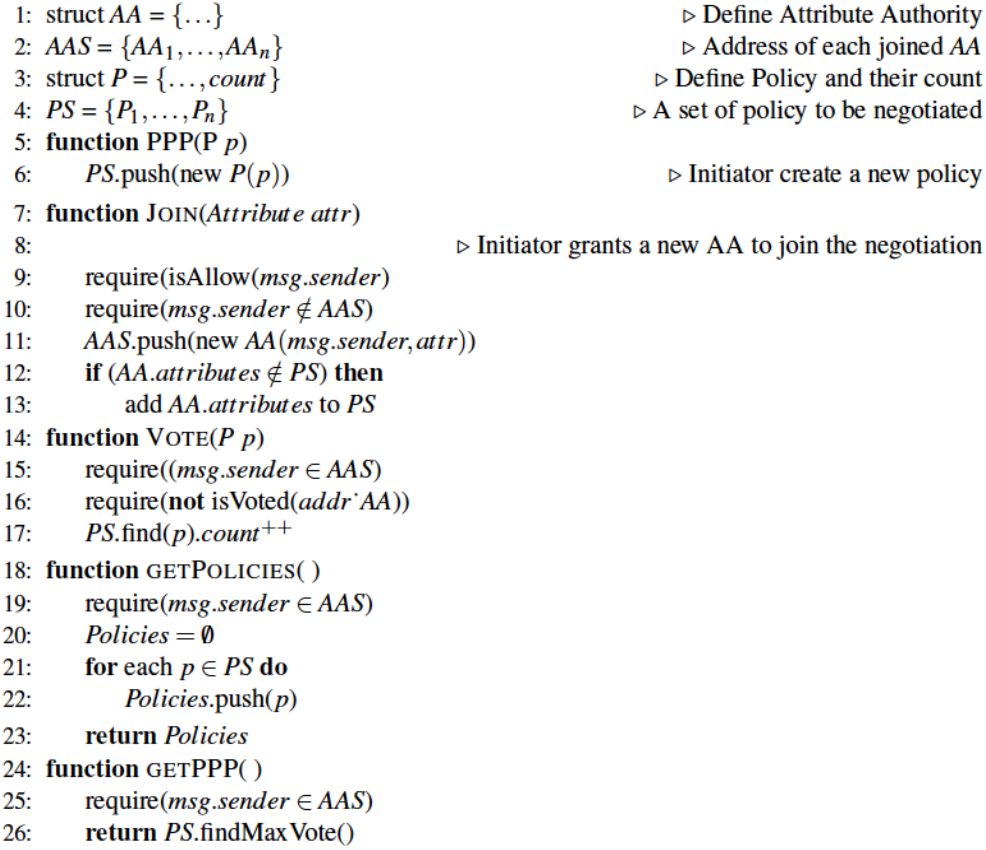
\includegraphics[scale=0.25]{pppcontract.png}
\caption{Pseudo-code of PPP Contract.}
\label{fig:pppcontract}
\end{figure}

\end{frame}

\begin{frame}[allowframebreaks]{ppSCM Contract}

\begin{itemize}

\item \textit{ppSCM} contract is a smart contract created by a supplier on a dedicated private blockchain.
\item It uses the negotiated policy from \textit{PPP} on a public blockchcain to create a contract for transactions involving supplier, buyer and carrier on the new created permission-based private blockchain.
\item The permission to access the private blockchain is controlled by the access control policy.
\item \textit{ppSCM} will maintain purchase orders and invoices for the same buyer and supplier on a dedicated private blockchain.
\item The data in purchase orders and invoices are protected by the selected access policy from \textit{PPP}. Only the parties with appropiated attributes can query or update the data via transactions.
\item When a buyer would like to purchase from a supplier, the supplier deploys \textit{ppSCM} smart contract exclusively for the buyer's account.
\item The buyer then put the purchse order on the supplier's \textit{ppSCM} with product name and quantity by calling \textit{sendOrder} function.
\item Through an event, so-called \textit{OrderSent}, the supplier could receive the order data and process it.
\item After received the purchase order, the supplier looks for the best shipping price on the carrier's smart contract.
\item The supplier sends the order price and shipment price to the buyer by calling \textit{sendPrice} and the buyer receives this through the event called \textit{PriceSent}.
\item The buyer performs the safe payment of the grand total (order price + shipment price) through the smart contract in the public blockchain by the \textit{SafepaySent()} event in the \textit{ppSCM}.
\item These coins goes to the smart contract account and waits there until the delivery.
\item After safe payment, the supplier sends the invoice with delivery date and some other data to the buyer by calling \textit{sentInvoice}. The buyer receives the invoice data through the event called \textit{InvoiceSent}.
\item The carrier, after delivery, marks the order as delivered on the \textit{ppSCM} smart contract by calling \textit{delivery} function.
\item The event \textit{OrderDelivery} then calls a smart contract in the public blockchain to payout the supplier for the order, and payout the carrier for the shipment.

\end{itemize}
\end {frame}
\begin{frame}{Pseudo-code of ppSCM Contract pt. 1}
\begin{figure}
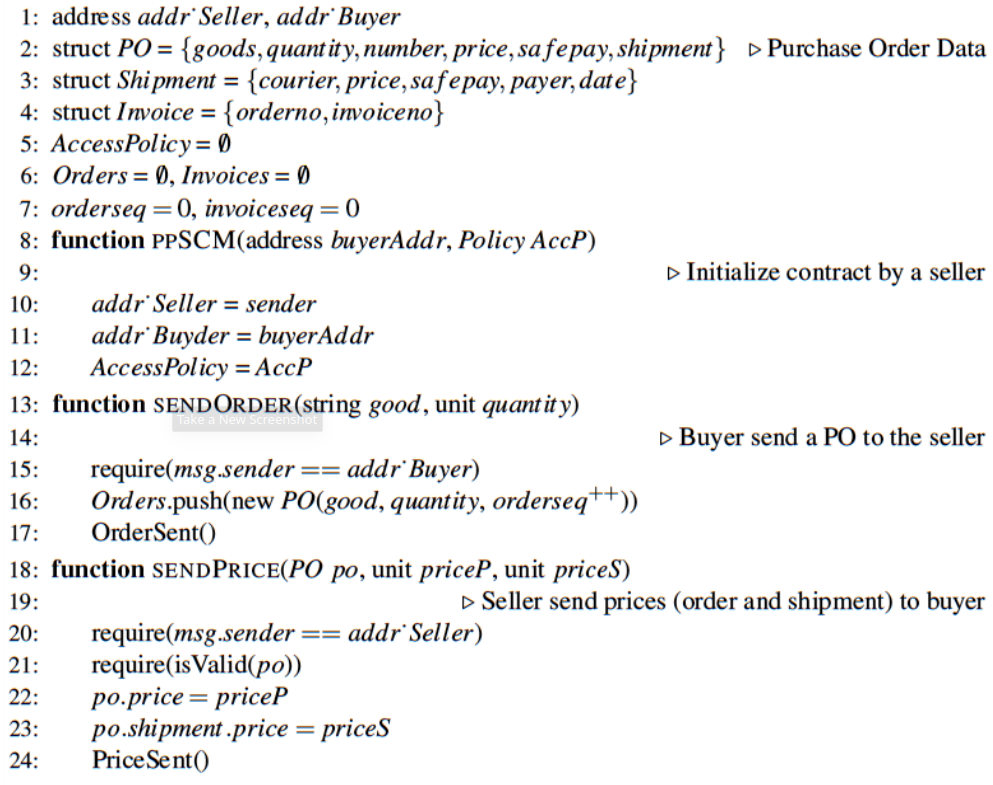
\includegraphics[scale=0.25]{ppscmcontract1.png}
\caption{Pseudo-code of first part of ppSCM Contract.}
\label{ppscm1}
\end{figure}
\end{frame}
\begin{frame}{Pseudo-code of ppSCM Contract pt. 2}
\begin{figure}
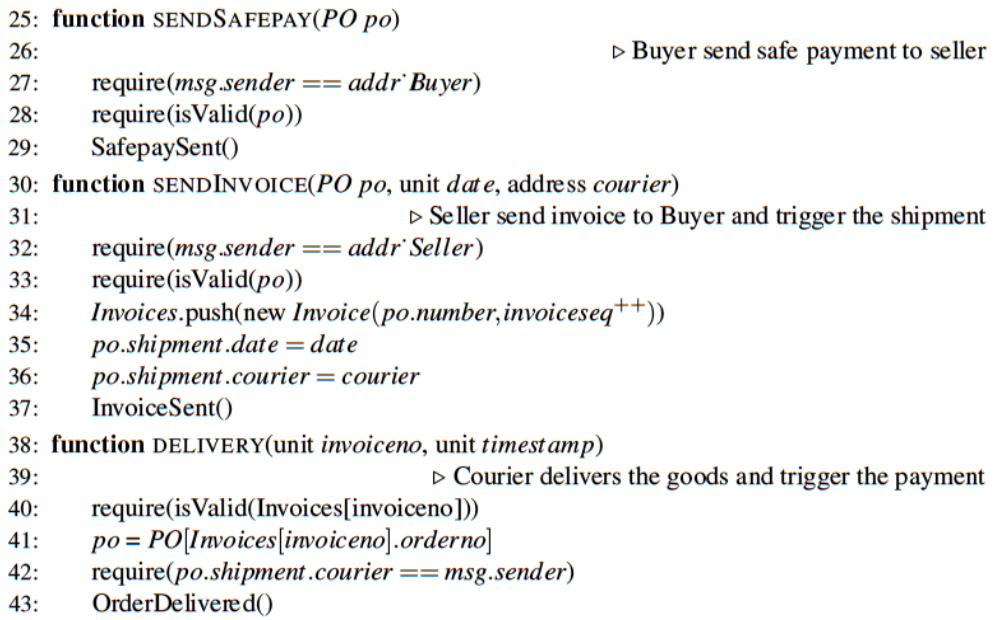
\includegraphics[scale=0.3]{ppscmcontract2.png}
\caption{Pseudo-code of second part of ppSCM Contract.}
\label{ppscm2}
\end{figure}

\end{frame}

\begin{frame}[allowframebreaks]{Policy-Based Data Privacy Protection}

\begin{figure}
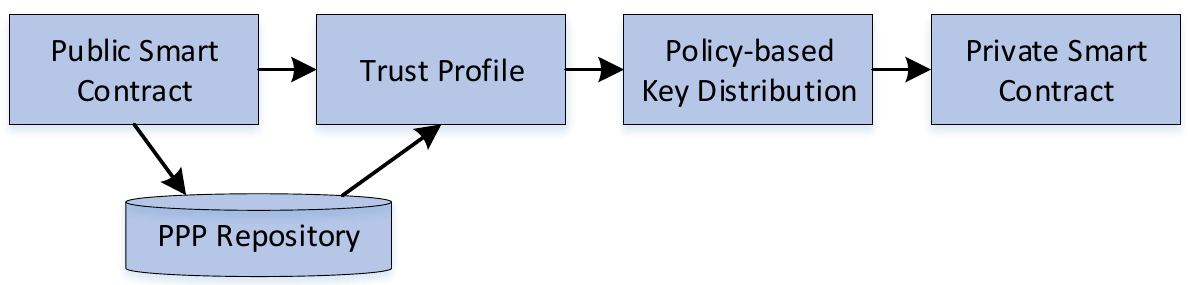
\includegraphics[scale=0.3]{pppdataprotection.png}
\caption{Trust and policy management procedure}
\label{ppptrustpolicy}
\end{figure}

For each private blockchain construction, we need to set up or choose a trust profile, i.e., either derived from a public smart contract to generate a PPP or reuse a previously establish PPP.
\framebreak
A PPP is built based on the following data structure:
\begin{itemize}
\item D1: A set of Global Parameters (GP) provides the global parameters that all ABE users need to use for key generation, encryption, and decryption.
\item D2: An array of identities of authorities ({GID}) and their associate public parameters $\{MPK\}$ and/or federated public parameters $\hat{MPK}$, and each parameter associated attributes $\{MPK\}$, $\hat{MPK} \rightarrow \{A\}$. The mapping between public parameters and attributes allow each private blockchain participant to select which public parameters to use in the ABE \textbf{Encrypt} procedure.
\item D3: A set of policy examples that can be used for each of smart contract transaction during the private blockchain construction.

\end{itemize}

PPP is built using smart contracts over public blockchain (Figure \ref{fig:pppcontract}), and thus they are searchable. A public directory service can be used to store established PPP. The PPP can be \textbf{resued} as a template for a new private blockchain.\\
In addition, when creating a new private blockchain, the participant can initiate an \textbf{update smart contract} to update the authority list and associated attributes.

\end{frame}

\begin{frame}[allowframebreaks]{Private Key Distribution}

\begin{itemize}

\item Once a PPP is determined and trusted authorities are known, a private key distribution procedure is conducted as an off-chain procedure.
\item The key distribution can be initiated by either a private blockchain participant or a trust authority.
\item  Using existing public key exchange protocols can allow the participants to derive private keys corresponding to each assigned attribute.
\item Some of the attributes may need to get a capability certificate from a trusted authority when applying for a private key.
\item A capability certificate is usually a digitally signed document to prove the requester has the capability to conduct a business function, e.g., professional certificates, bank certificates, business type certificates, etc.
\item  Each certificate should be digitally signed by well-known certificate issuers on requestor’s GID.
\item Then, the trusted authorities can use \textbf{KenGen} or \textbf{Federated KeyGen} to generate private keys for distribution.
\item The key distribution is an off-chain procedure and can be done offline.
\item Any existing public key or shared key-based key distribution schemes can be used.

\end{itemize}

\end{frame}

\begin{frame}[allowframebreaks]{Data Object Encryption and Decryption}

\begin{figure}
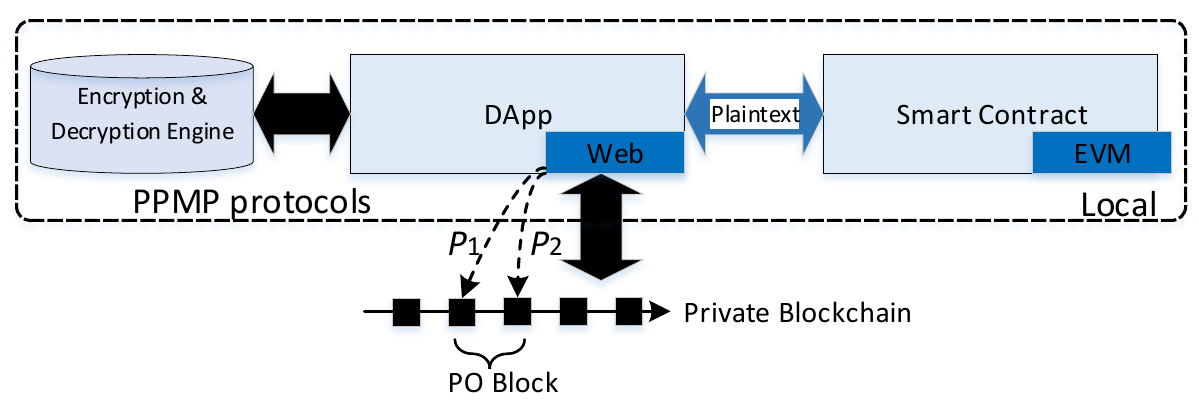
\includegraphics[scale=0.3]{dataobjectencdec.png}
\caption{Data object encryption and decryption.}
\label{fig:datobjencdec}
\end{figure}

\begin{itemize}

\item The data access protocol is specified in PPMP protocol.
\item The data object operation diagram is presented in Figure \ref{fig:datobjencdec}.
\item Both DApp (a web-based app) and smart contract (running within an Ethereum Virtual Machine (EVM)) run locally on a user's site.
\item The ABE encryption/decryption engine is also interfaced to the DApp locally. The encryption and decryption are performed between the DApp and the blockchain, and the encryption/decryption engine.
\item The data object granularity is determined by access control policies.
\item Using the policy provided in \textit{Security Policy I}: 
$\mathcal{P}1=$\textit{The pricing and quantity can be accessed by the supplier and the buyer}.
\item $\mathcal{P}1$ is an example to specify the data protection when creating the PO.
\item The PPMP message that will be used on DApp, which runs on ABE enc/dec engine to create the PO blockchain block and can be written as:\\
$PPMP(T, \{a\}, \mathcal{P},c ,s, o) =$\\
$= T_{PO}: \{buyer, supplier\} \rightarrow price\&quantity|_{create:\mathcal{P}1,E}$.
\item PO should also contain an address information for shipment.
\item If the data access policy is $\mathcal{P}2=$\textit{The shipment address information can be accessed by the buyer and the carrier.}, then the PPMP message can be:\\
$PPMP(T, \{a\}, \mathcal{P},c ,s, o) =$\\
$= T_{PO}: \{buyer, carrier\} \rightarrow shipping address|_{create:\mathcal{P}2,E}$.
\item The PO example presents two data access control policies $\mathcal{P}1$ and $\mathcal{P}2$ are involved, and thus on the blockchain, there should be at least two transactions corresponding to $\mathcal{P}1$ and $\mathcal{P}2$, respectively.
\item The granularity of encrypted block on the blockchain is determined by using the same data access control policy without needing to create two different DEKs.
\item Technically, we can combine $\mathcal{P}1$ and $\mathcal{P}2$ as one policy, however, there is no way to use one DEK to protect the data content to fulfill both of them.
\item  Other crypto actions such as decryption can be similarly created based on the PO example.
\item The crypto currency involved functions can be achieved by using public blockchain’s payment channel approach .
\end{itemize}

\end{frame}

\section{PoP Operation and Performance Analysis}
\begin{frame}[allowframebreaks]{Complexity Analysis}
\begin{table}
\begin{tabular}{|c|c|}
\hline 
Schemes & Complexity \\ 
\hline 
Setup & $2|U_i|$ \\ 
\hline 
KeyGen & $2|S|$ \\ 
\hline 
Encrypt & $5n$\textbf{E}$+1$ \\ 
\hline 
Decrypt & $2n$\textbf{P}$+ n$\textbf{E} \\ 
\hline 
\end{tabular}
\caption{Computation complexity comparison in terms of the number of pairing operations.}
\label{tab:compcomplex1}
\end{table}

\begin{itemize}
\item \textbf{E} and \textbf{P} represents exponentiation and pairing respectively.
\item $U_i$ indicates the set of attributes managed by a certain attribute authority.
\item S represents the set of attributes assigned to a user.
\item $n$ is the number of rows of the linear secret sharing matrix used in the encryption and decryption algorithm.
\end{itemize}

\begin{table}
\begin{tabular}{|c|c|c|c|}
\hline 
Schemes & DABE & device & edge node \\ 
\hline 
Setup & $2|U_i|$ & $2|U_i|$ & 0 \\ 
\hline 
KeyGen & $2|S|$ & $2|S|$ & 0 \\ 
\hline 
Encrypt & $5n$\textbf{E}$+1$ & $2n$\textbf{E}$+1$ & $3n$\textbf{E} \\ 
\hline 
Decrypt & $2n$\textbf{P}$+ n$\textbf{E} & $n$\textbf{P}$+ n$\textbf{E} & $n$\textbf{P} \\ 
\hline 
\end{tabular} 
\caption{Complexity of the algorithms of the presented scheme.}
\label{tab:compcomplex2}

\end{table}

\begin{itemize}
\item Table \ref{tab:compcomplex2} compares the complexity of the original algorithms and the scheme with Offloaded encryption and decryption.
\item It is seen that for the encryption the edge node is able to do more than half of the computational work.
\item As for the decryption, the edge node will share half number of the pairing operations.
\item Since the main complexity is caused by exponentiation and pairing, we only count the number of these two operations
\end{itemize}

\end{frame}

\begin{frame}{Computation Evaluation}
The evaluation is based on Charm, i.e., a python library for pairing-based cryptography. The evaluation environment is a VM on top of Intel Xeon CPU E5-2650 v2 @ 2.60hZ. Two virtual CPU, 4GB RAM and 80GB hard disk are assigned for this VM.\\
The performance evaluation of setup, keygen, encrypt and decrypt is presented from Figure \textbf{\ref{fig:setuptime}} to Figure \textbf{\ref{fig:decrypttime}}.\\
Figure \textbf{\ref{fig:enctimeol}} and Figure \textbf{\ref{fig:dectimeol}} compare the computation overhead between the edge node and the user's end.

\end{frame}

\begin{frame}{Setup and KeyGen times}

\begin{figure}
	\begin{subfigure}{.5\textwidth}
		\centering
		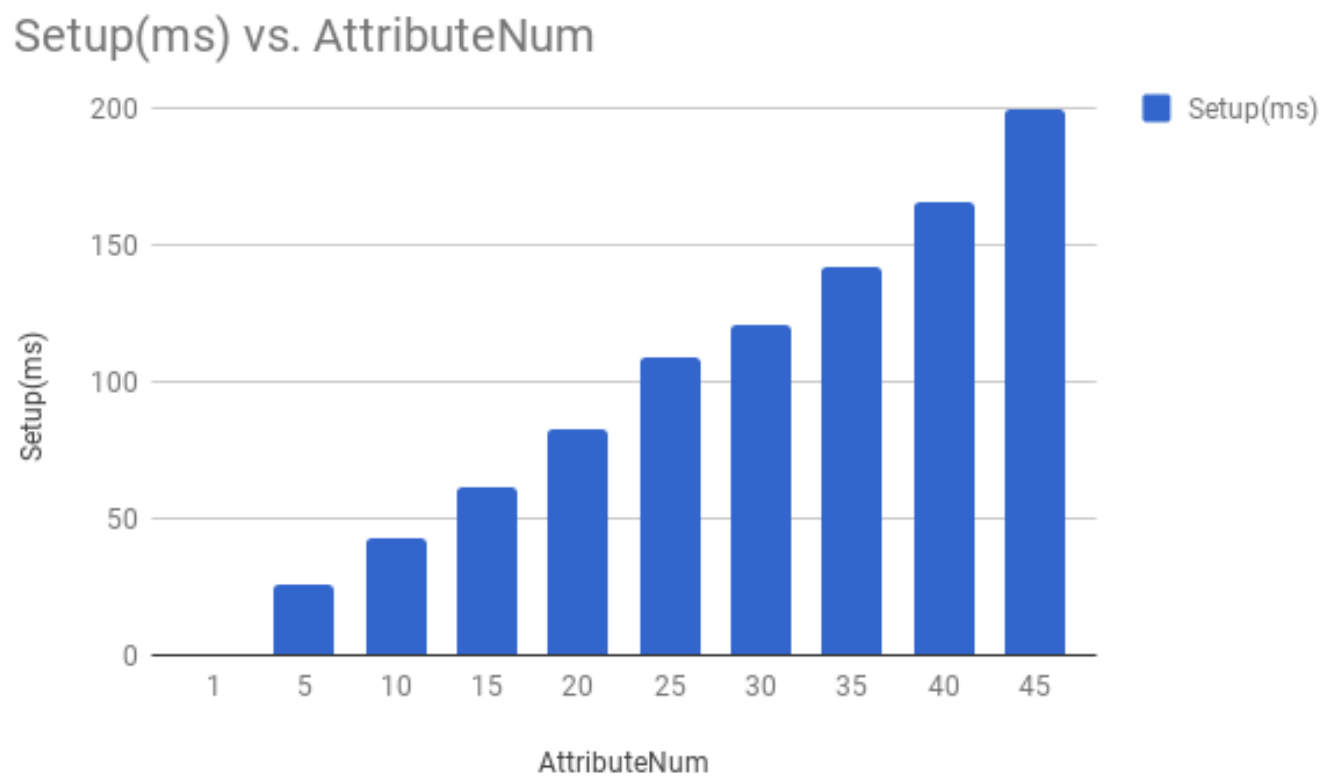
\includegraphics[scale=0.17]{setuptime.png}
		\caption{Setup time.}
		\label{fig:setuptime}
	\end{subfigure}%
	\begin{subfigure}{.5\textwidth}
		\centering
		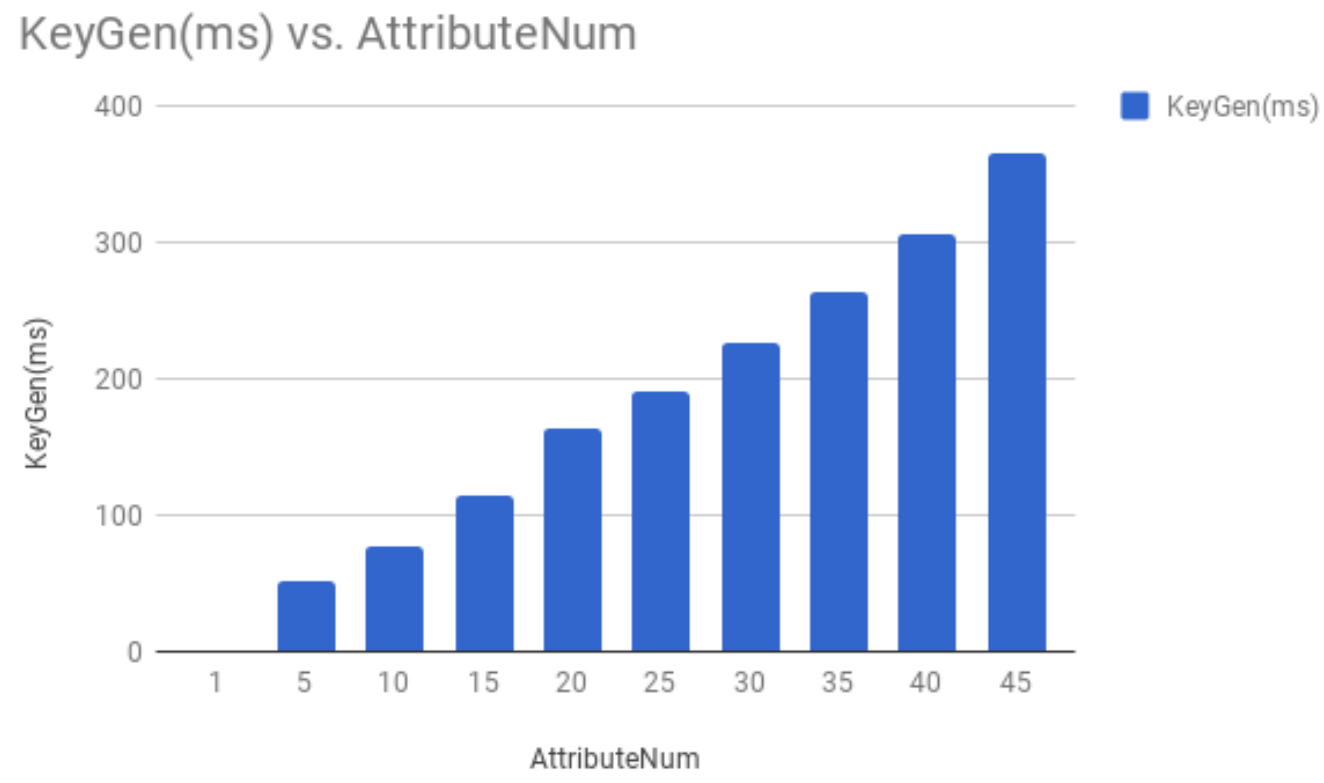
\includegraphics[scale=0.17]{keygentime.png}
		\caption{KeyGen time.}
		\label{fig:keygentime}
	\end{subfigure}
	\caption{Setup and KeyGen times.}
\end{figure}

\end{frame}

\begin{frame}{Encryption and Decryption times}

\begin{figure}
	\begin{subfigure}{.5\textwidth}
		\centering
		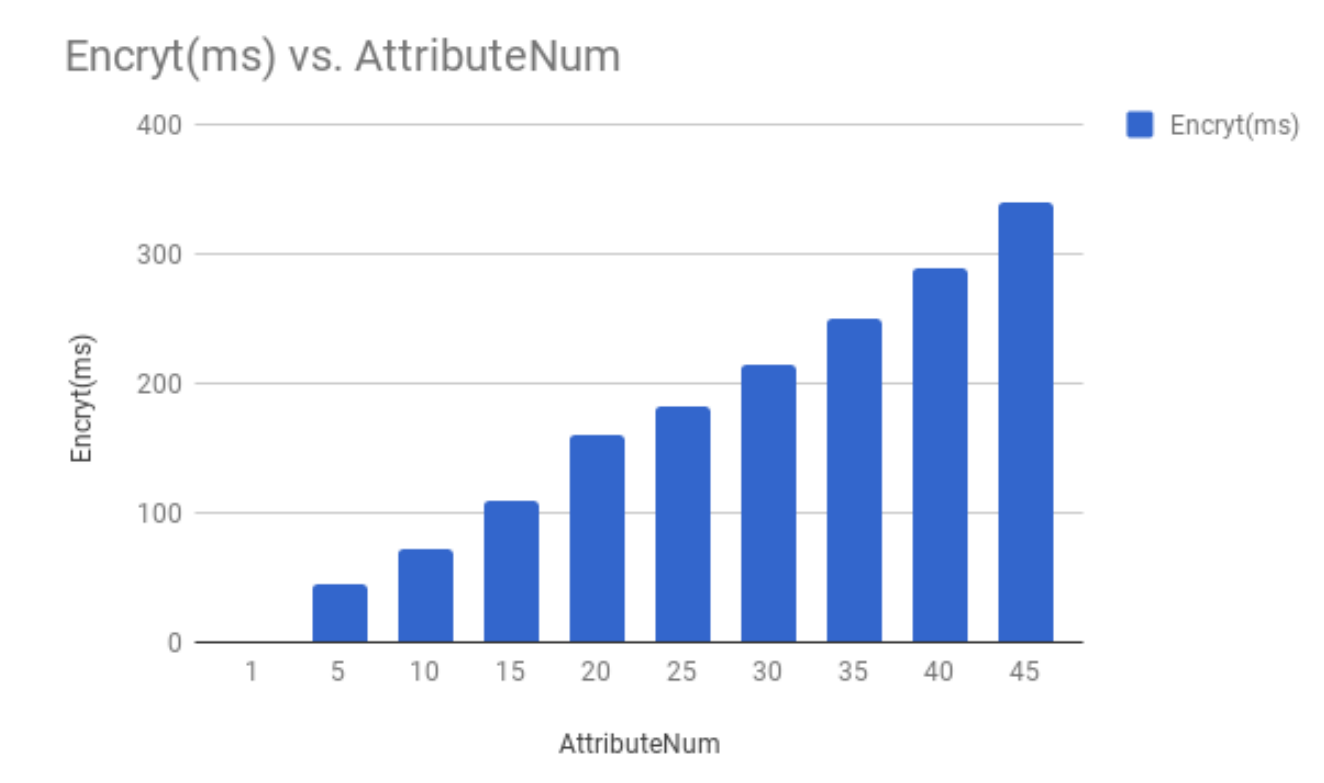
\includegraphics[scale=0.17]{encrypttime.png}
		\caption{Encryption time.}
		\label{fig:encrypttime}
	\end{subfigure}%
	\begin{subfigure}{.5\textwidth}
		\centering
		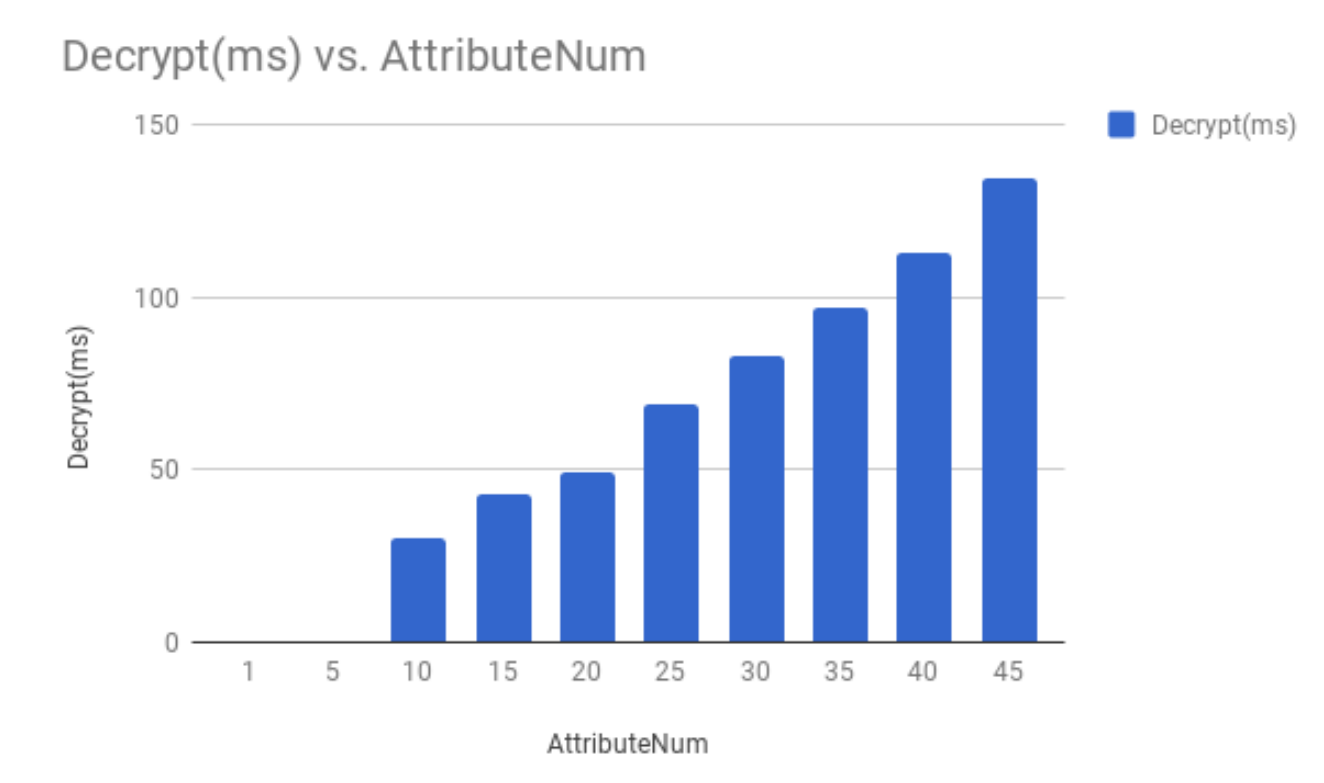
\includegraphics[scale=0.17]{decrypttime.png}	
		\caption{Decryption time.}
		\label{fig:decrypttime}
	\end{subfigure}
	\caption{Encryption and Decryption times.}
\end{figure}

\end{frame}

\begin{frame}{Computation Overhead with Offloading}

\begin{figure}
	\begin{subfigure}{.5\textwidth}
		\centering
		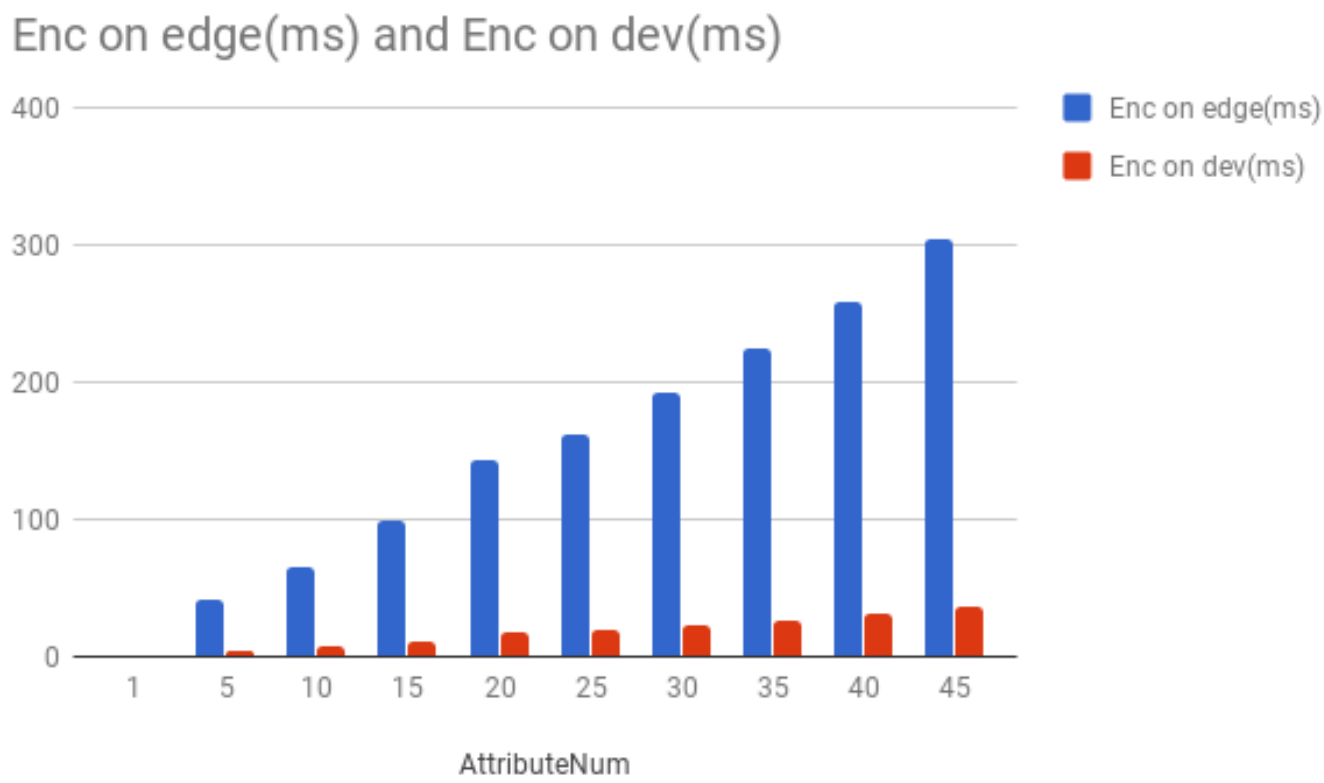
\includegraphics[scale=0.17]{olenctime.png}
		\caption{Encryption time.}
		\label{fig:enctimeol}
	\end{subfigure}%
	\begin{subfigure}{.5\textwidth}
		\centering
		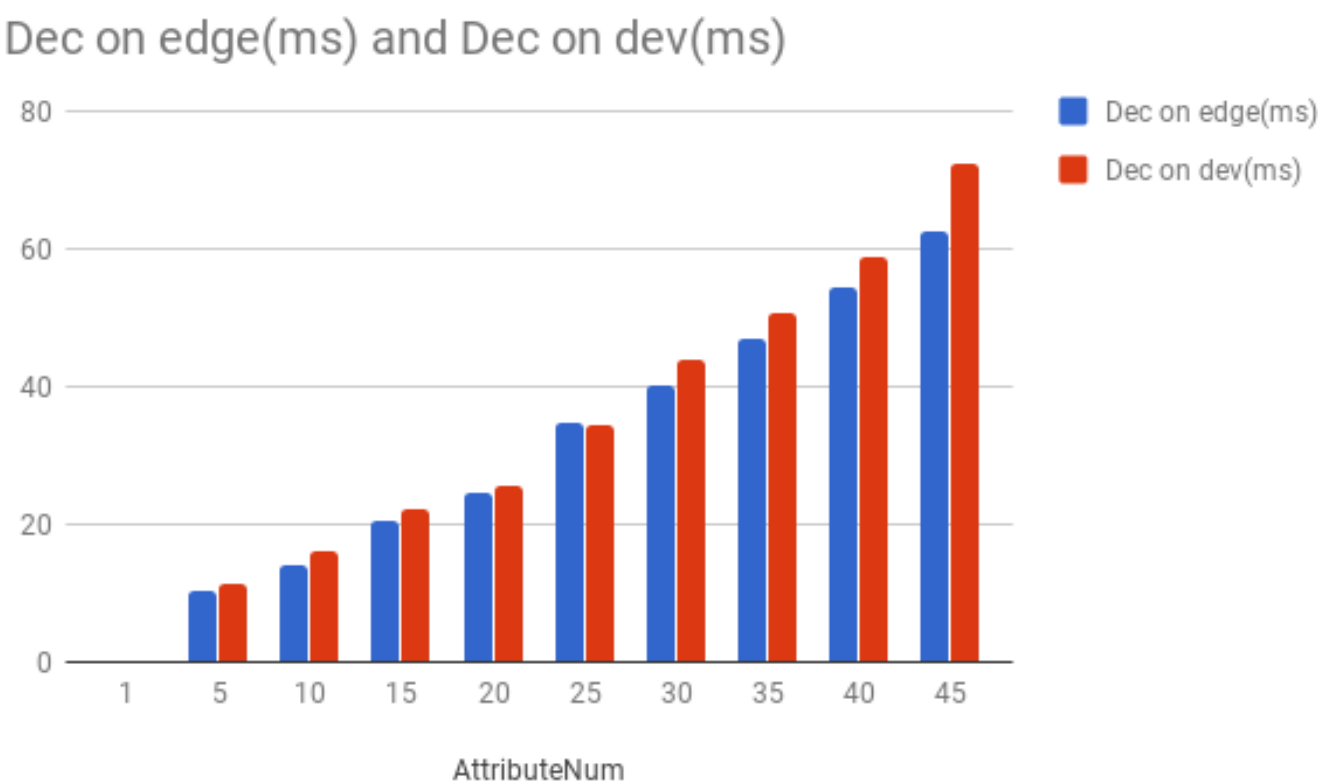
\includegraphics[scale=0.17]{oldectime.png}
		\caption{Decryption time.}
		\label{fig:dectimeol}
	\end{subfigure}
	\caption{Computation overhead between the edge node and the user's end.}
\end{figure}

\end{frame}

\begin{frame}[allowframebreaks]{Security Analysis}

\begin{itemize}
\item The presented ABE scheme is based on Lewko's scheme from \cite{lewkowaters}.
\item Lewko's scheme is proved to be secure against
	\begin{itemize}
	\item multiple $(n - 1)$ trusted authority collusion attack;
	\item collusion among users.
	\end{itemize}
\item The solution extends Lewko's scheme to \textbf{Federated Authority Setup} and \textbf{Federated KeyGen}.
\item The federated setup and key generation algorithm does not cause security issue and break the collusion problem provided by Lewko's scheme.
\item We have the following theorem:
\end{itemize}
\begin{theorem}
The presented scheme is resistant against attacks from colluded attribute authorities.
\end{theorem}
\framebreak
\begin{proof}
Assume that $n - 1$ attribute authorities in \textit{AAS} except for one attribute authority \textit{AA'} colluded, each of which provides the value $\alpha_j$ and $y_j$ $(AA_j \in AAS$ and $AA_j \not = AA')$. We denote the set of colluded attribute authorities as CAA. To compromise the presented scheme, the colluded atuthorities need to obtain the value of $\alpha = \Sigma_{j\in AAS}\alpha_j$ and $y = \Sigma_{j \in AAS}y_j$. However, they can only get the value of $\alpha' = \Sigma_{j \in CAA} \alpha_j$ and $y' = \Sigma_{j \in CAA}y_j$. Assume that they successfully calculate the value $\alpha$ and $y$ with access to $\alpha', y', e(g_1,g_1)^{\alpha_j}$ and $g_1^{y_j}(AA_j = AA')$, $\Rightarrow$ the colluded attribute authorities solved well known computationally difficult problem - discrete logarithm problem $\Rightarrow$ contradiction $\Rightarrow$ the presented scheme is resistant against the colluded attribute authorities.
\end{proof}

\end{frame}
\begin{frame}{Collusion Resistance Summary}

\begin{itemize}
\item For an adversary to compromise the system during federated setup and private key generation, the values $\Sigma_{j = 1}^n=\alpha_j$ and $\Sigma_{j = 1}^n y_j$ must be obtained.
\item Because the discrete logarithm problem is difficult in terms of a prime group that is big, the adversary cannot obtain each individual value $\alpha_j$ and $y_j$.
\item The only way to do this is attribute authority collusion.
\item However, it is only when all of the attribute authority colludes together can the private secret get leaked.
\item If the number of colluding attribute authority is $n - 1$ or fewer than that, the presented federated algorithms are resistant against collusion attacks.
\end{itemize}

\end{frame}

\begin{frame}[allowframebreaks]{Security Analysis of he Scheme with Offloaded Encryption and Decryption}
\begin{itemize}
\item In the Offloaded encryption algorithm, both the message \textit{M} and related information of the shared secret \textit{s} is leaked to the edge node.
\item The edge node is capable to help offload the computation overhead and also knows nothing about the encrypted message.
\item In the decryption algorithm, the edge node is only responsible for the private key unrelated computation, i.e., $C_{1,x}\cdot e(H(GID),C_{3,x})$.
\item Therefore, the private key is not leaked to the edge node, while the edge node can still help do the decryption.
\item Easily proved that offloaded scheme is secure if the original scheme is secure.

\end{itemize}
\end{frame}

\begin{frame}{Main feature comparison with existing major privacy preserving solutions}

\begin{figure}
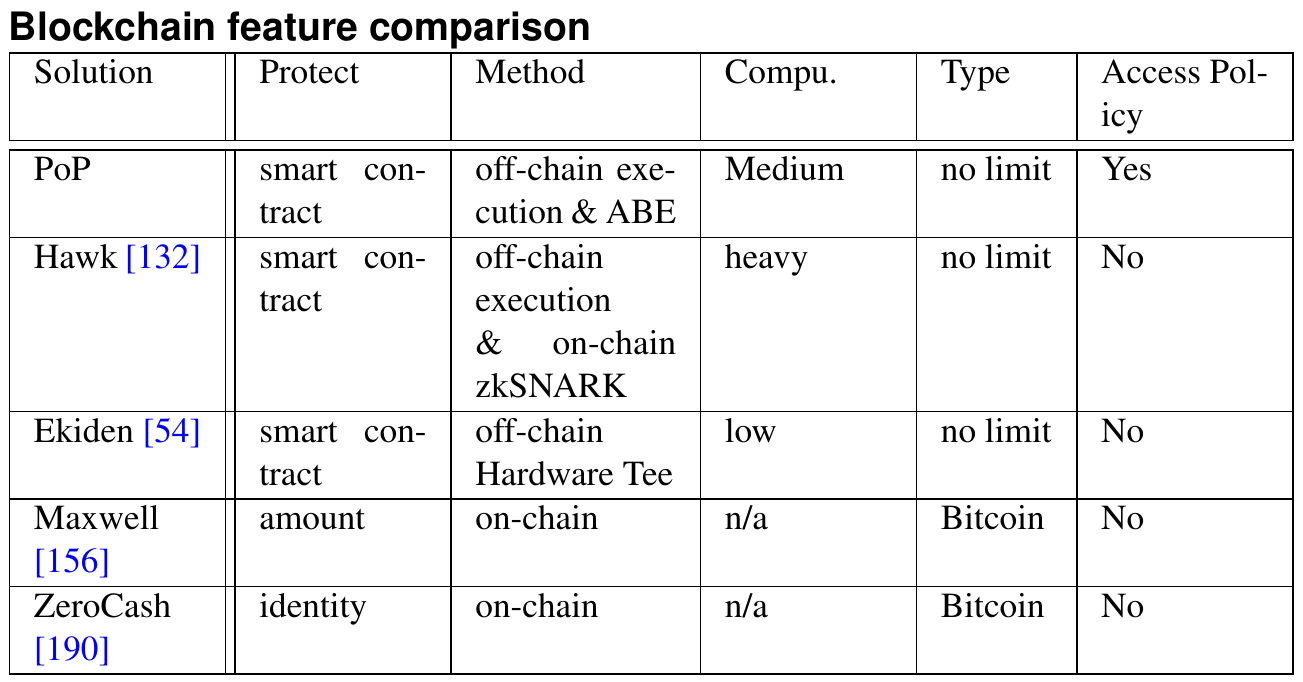
\includegraphics[scale=0.3]{blockchainfeatcomp.png}
\end{figure}

\end{frame}

\section{Summary}
\begin{frame}{Summary}
\begin{itemize}
	\item Presented a blockchain solution on how to build private blockchains over public blockchains - PoPs.
	\item Presented a set of messaging and smart contract protocols - to illustrate privacy-preserving functions of PoP.
	\item Use of a supply-chain procurement procedure example to illustrate how PoP works.
	\item A starting point for research and development for the next step:
	\begin{itemize}
		\item More functional-rich policy-based access control solutions should be considered: ex. policy/attributes expiration.
		\item The presented smart contract only focuses on PPP establishment and procurement. Other smart contracts such as cancellation/revocation of a contract should be investigated.
	\end{itemize}
\end{itemize}
\end{frame}

\begin{frame}[allowframebreaks]{References}
\printbibliography
\end{frame}

\end{document}